\subsection{A fejrész elemei}

%62
\begin{frame}
  A \texttt{<head>} tartalmazza a HTML oldal metaadatait. HTML5-től elhagyható, de javasolt használni. Beágyazható elemek:
  \begin{description}[m]
    \item[\texttt{<title>}] \hfill \\ A dokumentum címe, kötelező.
    \item[\texttt{<style>}] \hfill \\ CSS stílusok, formázás megadása; ált. jobb külön fájlba helyezni, ld. később 
    \item[\texttt{<base>}] \hfill \\ A relatív URL-ek a \texttt{href} értéke alapján lesznek értelmezve. A \texttt{target} más elemek \texttt{target} attribútumának alapértelmezett értékét adja meg.
  \end{description}
\end{frame}

%63
\begin{frame}
  \begin{description}[m]
    \item[\texttt{<link>}] \hfill \\ Külső erőforrás és a dokumentum kapcsolatát adja meg. Jellemző alkalmazásai:
    \begin{itemize}
      \item Stíluslap meghatározása: \texttt{href}-ben a CSS fájl URL-je, \texttt{rel} (relationship) \emph{stylesheet}, a \texttt{type} \emph{text/css} értékű.
      \item Ikon (favicon = favorite icon) beállítás: \texttt{href}-ben az ikon URL-je, \texttt{rel} \emph{icon}, a \texttt{type} pl. \emph{image/svg+xml} értékű. (További \hiv{\href{https://en.wikipedia.org/wiki/Favicon}{részletek}}.)
    \end{itemize}
    \item[\texttt{<meta>}] \hfill \\ HTTP fejlécek kulcs (\texttt{http-equiv} attribútum) - érték (\texttt{content} attribútum) párok formájában történő megadására. Jellemző kulcsok:
    \begin{itemize}
      \item \emph{content-type}, a MIME típus és karakterkódolás megadására: \texttt{content="text/html; charset=UTF-8"} $\to$ HTML5-től: csak a \texttt{charset="UTF-8"} attribútummal
      \item \emph{refresh}, automatikus újratöltés, pl. percenként: \texttt{content="60"}
    \end{itemize}
  \end{description}
\end{frame}

%64
\begin{frame}
  \begin{description}[m]
    \item[\texttt{<meta>}] \hfill \\ Metaadatok kulcs (\texttt{name} attribútum) - érték (\texttt{content} attribútum) párok formájában történő megadására. Jellemző kulcsok:
    \begin{itemize}
      \item \emph{description}, weboldal általános leírása
      \item \emph{keywords}, kulcsszavak keresőmotoroknak az oldal tartalmához kapcsolódóan
      \item \emph{author}, szerző
      \item \emph{viewport}, nézetablak beállítás, \texttt{content="width=device-width, initial-scale=1.0"}. Probléma: mobil eszközök nagy felbontásúak, de kis méretűek, számítógép-kijelzőre optimalizált oldalak gyenge felhasználói élménnyel használhatók. \emph{width=device-width}: a nézetablak szélessége alkalmazkodik az eszköz szélességéhez. \emph{initial-scale=1.0} nagyítás kezdeti értéke. \hiv{\href{https://www.quirksmode.org/mobile/viewports2.html}{Részletek}}
    \end{itemize}
  \end{description}
\end{frame}

%65
\begin{frame}
  \begin{description}[m]
    \item[\texttt{<script>}] \hfill \\ JavaScript programok megadására; előnyösebb a \texttt{<body>} végébe tenni (DOM felépül, az oldalbetöltést a JS kód nem lassítja).
    \item[\texttt{<noscript>}] \hfill \\ JavaScript támogatás hiányában a közrezárt szöveget megjeleníti. HTML5-től a \texttt{body}-ba is kerülhet.
  \end{description}
  \vfill
  HTML5-től a \texttt{<html>}, \texttt{<head>} és \texttt{<body>} elemek elhagyhatók, de ezt nem ajánljuk.
\end{frame}

%66
\begin{frame}
  \begin{exampleblock}{\textattachfile{fejresz.html}{fejresz.html} (\textattachfile{fejresz/fejresz.css}{fejresz/fejresz.css}, \textattachfile{fejresz/fejresz.js}{fejresz/fejresz.js}, \textattachfile{fejresz/fejresz2.html}{fejresz/fejresz2.html})}
    \scriptsize
    \lstinputlisting[style=HTML,linerange={3-16},numbers=left,firstnumber=3]{fejresz.html}
  \end{exampleblock}
\end{frame}

%66
\begin{frame}
  \begin{exampleblock}{\textattachfile{fejresz.html}{fejresz.html}}
    \lstinputlisting[style=HTML,linerange={17-22},numbers=left,firstnumber=17]{fejresz.html}
  \end{exampleblock}
  \begin{columns}[T]
    \column{0.3\textwidth}
      \centering 
\includegraphics[width=\textwidth]{fejresz_vilagos.png}
    \column{0.3\textwidth}
      \centering 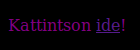
\includegraphics[width=\textwidth]{fejresz_sotet.png}
  \end{columns} 
\end{frame}

%67
\begin{frame}
  A \textattachfile{macska.txt}{macska.txt} fájlból kiindulva készítse el a \textattachfile{macska.html}{macska.html} oldalt az ábrának megfelelően!
  \begin{columns}[c]
    \column{0.65\textwidth}
      \begin{enumerate}
        \item Az oldal címe legyen \emph{Macska}!
        \item Az oldalt formázza meg a \textattachfile{macska.css}{macska.css} stíluslap segítségével!
        \item Jelenítse meg a \textattachfile[mimetype=image/png]{macska.png}{macska.png} fájlt ikonként (favicon)!
        \item A dokumentum kódolása UTF-8 szerint történjen!
        \item Készítsen \emph{ismertetőt}, adjon meg \emph{kulcsszavakat} a keresőmotorok számára! Adja meg a saját nevét \emph{szerzőként}!
        \item A nézetablak szélességét igazítsa a megjelenítő szélességéhez, a nagyítás legyen 1x-es!
        \item Szúrja be a macska képét (\textattachfile[mimetype=image/jpeg]{macska.jpeg}{macska.jpeg})!
      \end{enumerate}      
    \column{0.3\textwidth}
      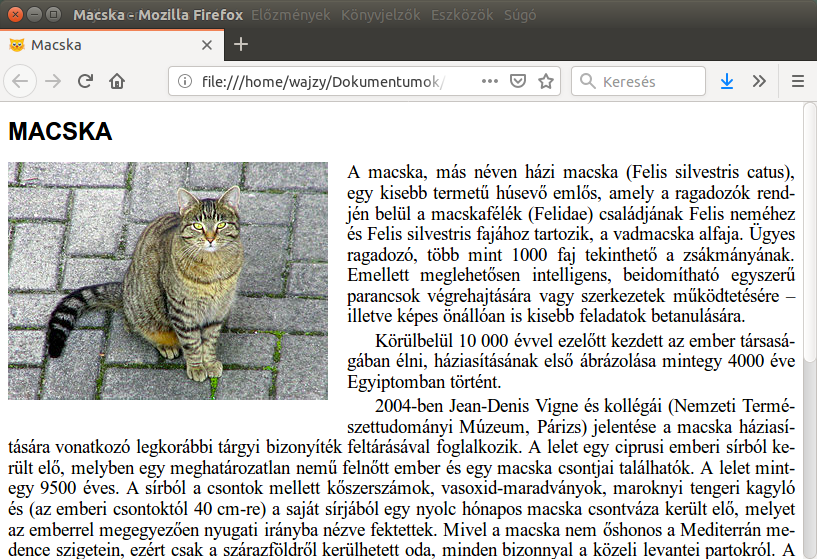
\includegraphics[width=\textwidth]{macska_screenshot.png}
  \end{columns} 
\end{frame}
